\chapter{Modeling}

\begin{figure}[hbtp]
	\centering
	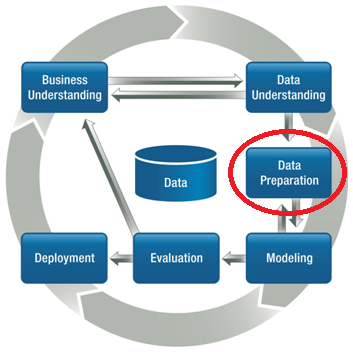
\includegraphics[width=0.5\textwidth]{./images/CRISPDM_3.png}
	\caption{CRISP-DM - Modeling}
	\label{CRISPDM_4}
\end{figure}

\section{Tecnica di Modeling}
Ai fini della classificazione, si è deciso di modellare il dataset realizzando un albero di decisione funzionale. In particolare si è utilizzato l'algoritmo \textbf{FT} (\emph{\textbf{F}unctional \textbf{T}ree}).

\section{Rappresentazione del Modello}
L'algoritmo Functional Tree è un algoritmo di classificazione basato sulla costruzione di alberi 'funzionali', i quali potrebbero avere funzioni di regressione logistica ai nodi e/o alle foglie interne. L'algoritmo, cosi come descritto in \cite{Gama:2004:FT:990375.990395}, è in grado di gestire:
\begin{itemize}
	\item variabili target (binarie o multi-classe)
	\item attributi numerici
	\item attributi nominali
	\item missing values
\end{itemize}
%Classifier for building 'Functional trees', which are classification trees  that could have logistic regression functions at the inner nodes and/or leaves. The algorithm can deal with binary and multi-class target variables, numeric and nominal attributes and missing values.\cite{Gama2004}

\paragraph{Functional Trees}
\subparagraph{Growning phase}
	Dato un set di esempi e un modello di costruzione di nuovi attributi, l'algoritmo generale usato per la creazione dell'albero funzionale risulta essere molto simile all'algoritmo standard per la costruzione degli alberi decisionali, fatta eccezione per alcuni passaggi; In particolare, nella fase di growning, si andranno a creare nuovi attributi derivati dalla valorizzazione delle funzioni di classificazione/regressione costruite sulla base degli attributi originali. Ci sono alcuni aspetti di questo algoritmo che devono essere esplicitati. Innanzitutto il modello verrà costruito usando la funzione costruttore creata tramite l'ausilio degli esempi che ricadono in un determinato nodo. La funzione costruttore deve essere un classificatore o un regressore, a seconda della tipologia di task da risolvere. Ogni nuovo attributo è computato come valore predetto dalla funzione costruita per ogni esempio. In caso di classificazione, ogni nuovo valore di questo attributo sarà ottenuto calcolando la probabilità che quell'esempio appartenga a una delle classi date (\emph{LinearBayes Classifier} \cite{DBLP:conf/sbia/Gama00}; Per fare ciò, si andrà a utilizzare la funzione di merito di un albero univariato tenendo conto sempre dei valori originali degli attributi (i.e. \emph{Gain Ratio}). Una voltacrati, questi nuovi attributi verranno utilizzati per la creazione del modello finale. Inoltre, la cardinalità dei nuovi attributi da creare sarà pari al quantitativo di classi che si hanno a disposizione.
	Il modello costruito dall'algoritmo potrà avere due tipologie di nodi decisionali: 
	\begin{itemize}
		\item nodi basati sul test eseguiti su un attributo originale;
		\item nodi valorizzati sulla base della funzione costruita.
	\end{itemize} 
	Nel secondo caso, si andrà a usare un modello lineare generalizzato per costruire i nuovi attributi; in questo caso, ogni nuovo attributo è ottenuto tramite combinazione lineare degli attributi di partenza. I nodi decisionali basati sui nuovi attributi, pertanto, permettono di definire un piano di decisione multivariato.

%\begin{figure}[hbtp]
%	\centering
%	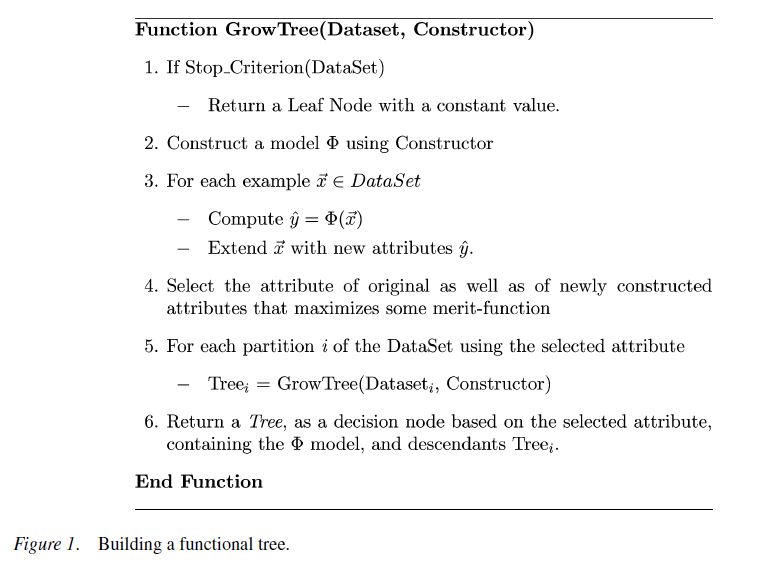
\includegraphics[width=0.9\textwidth]{./images/FunctionGrowTree.JPG}
%	\caption{Function GrowTree}
%\end{figure}

\lstset{style=customAlg}
\begin{algorithm}
	\caption{Function GrowTree(Dataset, Constructor)}
	\begin{lstlisting}
  If $Stop\_Criterion(DataSet)$
     Return a Leaf Node with a constant value.
  Construct a model $\Phi$ using Constructor
  For each example $\vec{x} \in DataSet$
     Compute $\hat y = \Phi(\vec{x})$
     Extend $\vec{x}$ with new attributes $\hat y$.
  Select the attribute of original as well as of newly constructed attributes that maximizes some merit-function
  For each partition $i$ of the DataSet using the selected attribute
     $Tree_{i} = GrowTree (Dataset_{i},Constructor)$
  Return a $Tree$, as a decision node based on the selected attribute, contaning the $\Phi$ model, and descendants $Tree_{i}$.
	\end{lstlisting}
\end{algorithm}

\subparagraph{Prune Phase}
	Una volta creato l'albero, si passerà alla fase di pruning in modo tale da ridurre l'overfitting dell'albero sul training set. L'algoritmo prevede la visita dell'albero usando un approccio bottom-up (Post-visita). Per ogni nodo non foglia vengono stimati due valori quantitativi: 
\begin{itemize}
	\item errore statico
	\item errore di Backed-up
\end{itemize}
L'\emph{errore statico} indica la probabilità di misclassification ad un nodo $v$ ignorando i suoi sottoalberi figli.
$$e(v) = P (class \neq C)|v$$
L'\emph{errore di backed-up}, invece, è la somma pesata della stima degli errori di tutti i sotto alberi del nodo corrente $v$. La stima dell'errore di ogni ramo è pesato usando la probabilità che un esempio appartenga al ramo.
$$E(T)=p_1E(T_1)+p_2E(T_2)+\dots$$ 
Se l'errore di backed-up dovesse essere maggiore o uguale dell'errore statico, il nodo verrà sostituito da una foglia avente come valore, il valore attribuito dalla classe di maggioranza del nodo.
L'errore a $T$ diventerà quindi il minimo trai 2 errori calcolati in precedenza.
$$ E(T) = \min \left( e \left( v \right), ~ \sum_i p_i E \left( T_i \right) \right) $$
L'aspetto fondamentale dell'algoritmo di potatura è l'errore stimato nella fase 1. Ad ogni nodo, sarà necessario stimare la probabilità dell'errore dato l'errore nel campione degli esempi che ricadono in questo nodo; inoltre, tale probabilità non può essere determinata con certezza. A tale scopo, per un dato livello di precisione, consideriamo un intervallo di confidenza $\left[L_{cf}~;~U_{cf}\right]$ con una probabilità di $1-cf$ che contenga l'errore reale. Cosi come in \cite{Quinlan:1993a}, il limite superiore dell'intervallo di confidenza ($U_{cf}$), ottenuto tramite errore di campionamento della distribuzione, sta a indicare la \emph{stima pessimistica} dell'errore reale. L'intervallo di confidenza per l'errore dipende dalla funzione di perdita\footnote{ La funzione di perdita riflette le conseguenze negative associate alla decisione "sbagliata"} usata. In caso di classificazione, con perdita 0-1, l'errore seguirà una distribuzione binomiale \cite{mitchellbook}.
Una procedura simile è utilizzata per stimare l'errore di costruzione ($Constructor\_Error$).

% \begin{figure}[hbtp]
% 	\centering
% 	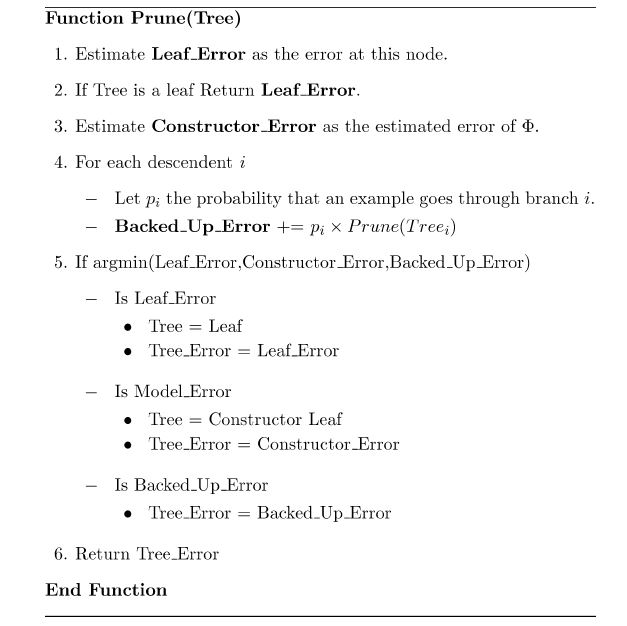
\includegraphics[width=0.5\textwidth]{./images/FunctionGrowTreePrune.JPG}
% 	\caption{Function GrowTree Prune}
% \end{figure}

\begin{algorithm}
	\caption{Function Prune (Tree)}
	\begin{lstlisting}
  Estimate Leaf_Error as the error at this node
  If Tree is leaf 
     Return Leaf_Error
  Estimate Constructor_Error as the estimated error of $\Phi$
  For each descendent $i$
     Let $p_i$ the probability that an example goes through branch $i$
     Backed_Up_Error $+= p_i \times Prune \left(Tree_i\right)$
  If argmin (Leaf_Error, Constructor_Error, Backed_up_error)
     Is Leaf_Error
        Tree = Leaf
        Tree_Error = Leaf_Error
     Is Model Error
        Tree = Constructor Leaf
        Tree_Error = Constructor_Error
     Is Backed_Up_Error
        Tree_Error = Backed_Up_Error
	\end{lstlisting}
\end{algorithm}
L'algoritmo di potatura sarà in grado di produrre due diversi tipi di foglie: 
\begin{itemize}
	\item Nodi foglia in grado di predire direttamente la classe da attribuire al nuovo esempio, nel caso in cui $$\min (E_{Backed\_Up}~,~E_{Static\_Error}) < E_{Constructor\_Error}$$	
	\item Nodi foglia contenenti la funzione costruttrice creata in fase di growing in quel nodo, nel caso in cui
	$$\min (E_{Backed\_Up}~,~E_{Static\_Error}) > E_{Constructor\_Error}$$
\end{itemize}
Si ottengono cosi due modelli concettualmente differenti in base a questa differenziazione, più un terzo modello ibrido.

\paragraph{Alberi funzionali ai soli nodi foglia}
\label{Alberi funzionali ai soli nodi foglia}
Utilizzando l'approccio FT-Leaves, il modello funzionale non viene utilizzato nei test per effettuare lo splitting, ma solo ed esclusivamente nelle foglie. In questo approccio, si restringe la selezione degli attributi di test ai soli attributi di partenza.
Questo è l'approccio utilizzato ad esempio nell'M5 di Quinlan \cite{DBLP:conf/icml/Quinlan93}, e nel sistema NBtree \cite{Kohavi1996}. 
Tuttavia, a ogni nodo viene costruita la funzione costruttore che verrà poi utilizzata nella fase di pruning dell'albero. In questo modo, tutti i nodi decisionali sono basati sugli attributi di partenza, ma anche i nodi foglia potrebbero contenere il modello costruttore se e solo se, nell'algoritmo di pruning, l'errore stimato del modello costruttore risulti essere inferiore sia all'errore di backed-up che all'errore statico. Un albero funzionale FT-Leaves divide lo spazio di input in iper-rettagoli. I dati in ogni regione vengono adattati usando la funzione costruttore.

\paragraph{Alberi funzionali ai soli nodi intermedi}
\label{Alberi funzionali ai soli nodi intermedi}
Utilizzando l'approccio FT-Inner, si otterranno degli alberi funzionali nel quale i modelli multivariati verranno usati esclusivamente ai nodi decisionali (nodi interni) e non verranno mai usati come classificatori nei nodi foglia. In questo caso, l'algoritmo di pruning verrà limitato alla sola scelta tra l'errore di  Backed-up e l'errore statico, facendo in modo che, nelle foglie, siano presenti solo i valori costanti utili alla classificazione diretta. Questo approccio è utilizzato in sistemi come LTREE (\cite{Gama97}). Un albero funzionale FT-Inner divide lo spazio di input in superfici decisionali oblique. I dati in ogni regione vengono adattati usando la costante che minimizzi la funzione di perdita data.
%\paragraph{Functional inner nodes only} We denote as FT-Inner the approach to functional trees where the multivariate models are used exclusively at decision nodes (internal nodes) and not used as classifiers in leaves. In our algorithm, restricting the pruning algorithm to choose only between the Backed-up-Error and the Static error generates this kind of model. In this case all leaves predict a constant value. This is the strategy used in systems like LMDT (Utgoff & Brodley, 1991), OC1 (Murthy, Kasif, & Salzberg, 1994), LTREE (Gama, 1997), and QUEST (Loh & Shih, 1997). A FT-Inner functional tree divides the input space into oblique decision surfaces. The data in each region is fitted with a constant that minimizes the given loss function. %
\paragraph{Alberi funzionali ibridi}
\label{FT Hybrid}
Combinando i due approcci descritti nei paragrafi precedenti, si ottiene un approccio ibrido nel quale è possibile avere il modello costruttore sia alle foglie che ai nodi intermedi senza nessun vincolo nè in fase di costruzione, nè in fase di potatura. Questo approccio prende il nome di \emph{FT model}.

\paragraph{Predire usando gli alberi funzionali}
Una volta ultimato l'algoritmo di creazione dell'albero (crescita e successiva potatura), questo viene usato per predire il valore di un attributo target su un esempio non classificato. Per fare ciò, l'esempio attraversa l'albero funzionale in modalità top-down (dal nodo radice al nodo foglia). Ad ogni nodo decisionale (inner node) dell'albero, il set di attributi dell'esempio viene esteso usando la funzione costruttore creata a quel nodo. Dopo questa espansione, il test decisionale del nodo viene applicato definendo il percorso che l'esempio dovrà seguire. Una volta che si raggiungerà un nodo foglia, l'esempio verrà classificato o secondo la costante associata al nodo foglia, oppure alla funzione costruttrice creata in quel nodo.

\section{Costruzione del Modello}
I parametri impostati per l'algoritmo Functional Tree in weka, saranno i seguenti:
\begin{multicols}{2}
\begin{itemize}
	\item binSplit: False
	\item debug: False
	\item errorOnProbabilities: False
	\item minNumInstances: 15
	\item \textbf{modelType}: \textbf{FT}
	\item numBoostingIterations: 15
	\item useAIC: False
	\item weightTrimBeta: 0.0
\end{itemize}
\end{multicols}

Il modello seguente è stato costruito usando la configurazione:
\begin{itemize}
	\item approccio ibrido FT (\ref{FT Hybrid})
	\item feature selection fatta con CfsSubsetEval (\ref{Feature Selection})
	\item sampling fatto con SMOTE (\ref{SMOTE})
\end{itemize}	
{\footnotesize
\begin{verbatim}
=== Run information ===

Scheme:     weka.classifiers.trees.FT -I 15 -F 0 -M 15 -W 0.0

Relation:   SPAM-weka.filters.supervised.instance.SMOTE-C0-K5-P100.0-S1-
            weka.filters.supervised.attribute.AttributeSelection-
            Eweka.attributeSelection.CfsSubsetEval-
            Sweka.attributeSelection.BestFirst -D 1 -N 5

Instances:  11112

Attributes: 53	
\end{verbatim}
\begin{multicols}{2}
	\begin{verbatim}
	id
	APPROVED_BY
	BASE64_ENC_TEXT
	BIG_FONT
	CLICK_BELOW
	CRON_ENV
	CTYPE_JUST_HTML
	DATE_IN_FUTURE_06_12
	DATE_IN_PAST_06_12
	DIET
	DOMAIN_4U2
	EXCHANGE_SERVER
	EXCUSE_14
	EXCUSE_3
	FAILURE_NOTICE_2
	FORGED_HOTMAIL_RCVD
	FORGED_YAHOO_RCVD
	FROM_ENDS_IN_NUMS
	HTML_FONT_COLOR_GRAY
	HTML_FONT_INVISIBLE
	HTML_WITH_BGCOLOR
	INVALID_DATE
	KNOWN_MAILING_LIST
	LINES_OF_YELLING
	MAILTO_TO_REMOVE
	MAY_BE_FORGED
	MIME_HTML_NO_CHARSET
	MISSING_MIMEOLE
	MORTGAGE_OBFU
	MSG_ID_ADDED_BY_MTA_2
	NORMAL_HTTP_TO_IP
	NO_REAL_NAME
	ONLY_COST
	PLING_QUERY
	QUOTED_EMAIL_TEXT
	REMOVE_PAGE
	RESENT_TO
	RISK_FREE
	SAVE_MONEY
	SIGNATURE_LONG_DENSE
	SIGNATURE_SHORT_SPARSE
	SPAM_PHRASE_00_01
	SPAM_PHRASE_08_13
	SUBJECT_MONTH
	SUBJ_ALL_CAPS
	TRACKER_ID
	UNSUB_PAGE
	USER_AGENT_PINE
	USER_AGENT_TONLINE
	USER_IN_WHITELIST
	WEB_BUGS
	X_ACCEPT_LANG
	target
	Test mode:10-fold cross-validation
	\end{verbatim}
\end{multicols}
\begin{verbatim}
	=== Classifier model (full training set) ===
	
	FT tree 
	------------------
	
	N0#1 <= 0.618916
	|   id <= 372407
	|   |   N0#3 <= 0.156641: FT_1:15/60 (4856)
	|   |   N0#3 > 0.156641
	|   |   |   N0#5 <= 0.825819
	|   |   |   |   N0#6 <= 0.513027: Class=1
	|   |   |   |   N0#6 > 0.513027: FT_3:15/90 (32)
	|   |   |   N0#5 > 0.825819: FT_4:15/75 (121)
	|   id > 372407: Class=0
	N0#1 > 0.618916
	|   N0#11 <= 0.865508: FT_6:15/45 (34)
	|   N0#11 > 0.865508
	|   |   N0#13 <= 0.995526
	|   |   |   N0#14 <= 0.973489: FT_7:15/75 (68)
	|   |   |   N0#14 > 0.973489: FT_8:15/75 (267)
	|   |   N0#13 > 0.995526: Class=0
	
	Number of Leaves  : 	9
	
	Size of the Tree : 	17
\end{verbatim}
\begin{multicols}{2}
	\begin{verbatim}
		FT_N0#1:
		Class 0 :
		-1.07 + 
		[id] * 0    +
		[BASE64_ENC_TEXT] * 2.03 +
		[BIG_FONT] * 0.88 +
		[CLICK_BELOW] * 0.9  +
		[CTYPE_JUST_HTML] * 2.17 +
		[FROM_ENDS_IN_NUMS] * 0.77 +
		[INVALID_DATE] * 1.11 +
		[MISSING_MIMEOLE] * 1.1  +
		[RESENT_TO] * 1.14 +
		[SPAM_PHRASE_00_01] * -1.44 +
		[USER_AGENT_PINE] * -0.72 +
		[WEB_BUGS] * 0.97 +
		[X_ACCEPT_LANG] * -0.72
		
		Class 1 :
		1.07 + 
		[id] * 0    +
		[BASE64_ENC_TEXT] * -2.03 +
		[BIG_FONT] * -0.88 +
		[CLICK_BELOW] * -0.9 +
		[CTYPE_JUST_HTML] * -2.17 +
		[FROM_ENDS_IN_NUMS] * -0.77 +
		[INVALID_DATE] * -1.11 +
		[MISSING_MIMEOLE] * -1.1 +
		[RESENT_TO] * -1.14 +
		[SPAM_PHRASE_00_01] * 1.44 +
		[USER_AGENT_PINE] * 0.72 +
		[WEB_BUGS] * -0.97 +
		[X_ACCEPT_LANG] * 0.72
		
		
		FT_N0#3:
		Class 0 :
		-1.52 + 
		[id] * 0    +
		[APPROVED_BY] * -0.53 +
		[BASE64_ENC_TEXT] * 3.04 +
		[BIG_FONT] * 0.88 +
		[CLICK_BELOW] * 0.9  +
		[CTYPE_JUST_HTML] * 4.01 +
		[DATE_IN_FUTURE_06_12] * 1.09 +
		[DIET] * 1.37 +
		[EXCHANGE_SERVER] * -0.52 +
		[EXCUSE_3] * 0.92 +
		[FORGED_HOTMAIL_RCVD] * 1.32 +
		[FORGED_YAHOO_RCVD] * 1.39 +
		[FROM_ENDS_IN_NUMS] * 0.77 +
		[HTML_FONT_COLOR_GRAY] * -0.97 +
		[INVALID_DATE] * 1.11 +
		[KNOWN_MAILING_LIST] * -0.68 +
		[MIME_HTML_NO_CHARSET] * 1.11 +
		[MISSING_MIMEOLE] * 2.16 +
		[MSG_ID_ADDED_BY_MTA_2] * 0.87 +
		[NORMAL_HTTP_TO_IP] * 1.53 +
		[ONLY_COST] * 1.44 +
		[PLING_QUERY] * 1.32 +
		[QUOTED_EMAIL_TEXT] * -1.06 +
		[REMOVE_PAGE] * 1.43 +
		[RESENT_TO] * 2.03 +
		[RISK_FREE] * 1.65 +
		[SPAM_PHRASE_00_01] * -0.76 +
		[SPAM_PHRASE_08_13] * 1.31 +
		[SUBJECT_MONTH] * -0.46 +
		[TRACKER_ID] * 1.3  +
		[USER_AGENT_PINE] * -1.26 +
		[WEB_BUGS] * 0.97 +
		[X_ACCEPT_LANG] * -1.37
		
		Class 1 :
		1.52 + 
		[id] * 0    +
		[APPROVED_BY] * 0.53 +
		[BASE64_ENC_TEXT] * -3.04 +
		[BIG_FONT] * -0.88 +
		[CLICK_BELOW] * -0.9 +
		[CTYPE_JUST_HTML] * -4.01 +
		[DATE_IN_FUTURE_06_12] * -1.09 +
		[DIET] * -1.37 +
		[EXCHANGE_SERVER] * 0.52 +
		[EXCUSE_3] * -0.92 +
		[FORGED_HOTMAIL_RCVD] * -1.32 +
		[FORGED_YAHOO_RCVD] * -1.39 +
		[FROM_ENDS_IN_NUMS] * -0.77 +
		[HTML_FONT_COLOR_GRAY] * 0.97 +
		[INVALID_DATE] * -1.11 +
		[KNOWN_MAILING_LIST] * 0.68 +
		[MIME_HTML_NO_CHARSET] * -1.11 +
		[MISSING_MIMEOLE] * -2.16 +
		[MSG_ID_ADDED_BY_MTA_2] * -0.87 +
		[NORMAL_HTTP_TO_IP] * -1.53 +
		[ONLY_COST] * -1.44 +
		[PLING_QUERY] * -1.32 +
		[QUOTED_EMAIL_TEXT] * 1.06 +
		[REMOVE_PAGE] * -1.43 +
		[RESENT_TO] * -2.03 +
		[RISK_FREE] * -1.65 +
		[SPAM_PHRASE_00_01] * 0.76 +
		[SPAM_PHRASE_08_13] * -1.31 +
		[SUBJECT_MONTH] * 0.46 +
		[TRACKER_ID] * -1.3 +
		[USER_AGENT_PINE] * 1.26 +
		[WEB_BUGS] * -0.97 +
		[X_ACCEPT_LANG] * 1.37
		
		FT_1:
		Class 0 :
		-1.95 + 
		[id] * 0    +
		[APPROVED_BY] * -1.04 +
		[BASE64_ENC_TEXT] * 3.04 +
		[BIG_FONT] * 0.88 +
		[CLICK_BELOW] * 4.97 +
		[CRON_ENV] * -0.54 +
		[CTYPE_JUST_HTML] * 31.85 +
		[DATE_IN_FUTURE_06_12] * 1.09 +
		[DIET] * 1.37 +
		[EXCHANGE_SERVER] * -0.52 +
		[EXCUSE_3] * 0.92 +
		[FORGED_HOTMAIL_RCVD] * 1.32 +
		[FORGED_YAHOO_RCVD] * 2.9  +
		[FROM_ENDS_IN_NUMS] * 0.36 +
		[HTML_FONT_COLOR_GRAY] * -0.97 +
		[INVALID_DATE] * 1.11 +
		[KNOWN_MAILING_LIST] * -0.68 +
		[MIME_HTML_NO_CHARSET] * 1.11 +
		[MISSING_MIMEOLE] * 2.16 +
		[MORTGAGE_OBFU] * 2.78 +
		[MSG_ID_ADDED_BY_MTA_2] * 0.87 +
		[NORMAL_HTTP_TO_IP] * 1.53 +
		[ONLY_COST] * 1.44 +
		[PLING_QUERY] * 1.32 +
		[QUOTED_EMAIL_TEXT] * -1.58 +
		[REMOVE_PAGE] * 1.43 +
		[RESENT_TO] * 2.03 +
		[RISK_FREE] * 1.65 +
		[SPAM_PHRASE_00_01] * -0.48 +
		[SPAM_PHRASE_08_13] * 1.31 +
		[SUBJECT_MONTH] * -1.83 +
		[TRACKER_ID] * 5.74 +
		[USER_AGENT_PINE] * -2.01 +
		[WEB_BUGS] * 0.97 +
		[X_ACCEPT_LANG] * -1.37
		
		Class 1 :
		1.95 + 
		[id] * 0    +
		[APPROVED_BY] * 1.04 +
		[BASE64_ENC_TEXT] * -3.04 +
		[BIG_FONT] * -0.88 +
		[CLICK_BELOW] * -4.97 +
		[CRON_ENV] * 0.54 +
		[CTYPE_JUST_HTML] * -31.85 +
		[DATE_IN_FUTURE_06_12] * -1.09 +
		[DIET] * -1.37 +
		[EXCHANGE_SERVER] * 0.52 +
		[EXCUSE_3] * -0.92 +
		[FORGED_HOTMAIL_RCVD] * -1.32 +
		[FORGED_YAHOO_RCVD] * -2.9 +
		[FROM_ENDS_IN_NUMS] * -0.36 +
		[HTML_FONT_COLOR_GRAY] * 0.97 +
		[INVALID_DATE] * -1.11 +
		[KNOWN_MAILING_LIST] * 0.68 +
		[MIME_HTML_NO_CHARSET] * -1.11 +
		[MISSING_MIMEOLE] * -2.16 +
		[MORTGAGE_OBFU] * -2.78 +
		[MSG_ID_ADDED_BY_MTA_2] * -0.87 +
		[NORMAL_HTTP_TO_IP] * -1.53 +
		[ONLY_COST] * -1.44 +
		[PLING_QUERY] * -1.32 +
		[QUOTED_EMAIL_TEXT] * 1.58 +
		[REMOVE_PAGE] * -1.43 +
		[RESENT_TO] * -2.03 +
		[RISK_FREE] * -1.65 +
		[SPAM_PHRASE_00_01] * 0.48 +
		[SPAM_PHRASE_08_13] * -1.31 +
		[SUBJECT_MONTH] * 1.83 +
		[TRACKER_ID] * -5.74 +
		[USER_AGENT_PINE] * 2.01 +
		[WEB_BUGS] * -0.97 +
		[X_ACCEPT_LANG] * 1.37
		
		FT_N0#5:
		Class 0 :
		-0.59 + 
		[APPROVED_BY] * -0.53 +
		[BASE64_ENC_TEXT] * 3.04 +
		[BIG_FONT] * 0.88 +
		[CLICK_BELOW] * 0.9  +
		[CTYPE_JUST_HTML] * 4.01 +
		[DATE_IN_FUTURE_06_12] * 1.09 +
		[DIET] * 2.22 +
		[EXCHANGE_SERVER] * -1.6 +
		[EXCUSE_3] * 0.92 +
		[FORGED_HOTMAIL_RCVD] * 1.32 +
		[FORGED_YAHOO_RCVD] * 0.96 +
		[FROM_ENDS_IN_NUMS] * 0.77 +
		[HTML_FONT_COLOR_GRAY] * -1.85 +
		[HTML_FONT_INVISIBLE] * -1 +
		[INVALID_DATE] * 1.11 +
		[KNOWN_MAILING_LIST] * -2.32 +
		[MIME_HTML_NO_CHARSET] * 1.11 +
		[MISSING_MIMEOLE] * 2.16 +
		[MSG_ID_ADDED_BY_MTA_2] * 0.39 +
		[NORMAL_HTTP_TO_IP] * 1.53 +
		[ONLY_COST] * 2.25 +
		[PLING_QUERY] * 2.37 +
		[QUOTED_EMAIL_TEXT] * -1.06 +
		[REMOVE_PAGE] * 1.43 +
		[RESENT_TO] * 2.03 +
		[RISK_FREE] * 2.57 +
		[SPAM_PHRASE_00_01] * -0.33 +
		[SPAM_PHRASE_08_13] * 1.31 +
		[SUBJECT_MONTH] * -0.46 +
		[TRACKER_ID] * 1.3  +
		[USER_AGENT_PINE] * -3.23 +
		[WEB_BUGS] * 0.97 +
		[X_ACCEPT_LANG] * -1.37
		
		Class 1 :
		0.59 + 
		[APPROVED_BY] * 0.53 +
		[BASE64_ENC_TEXT] * -3.04 +
		[BIG_FONT] * -0.88 +
		[CLICK_BELOW] * -0.9 +
		[CTYPE_JUST_HTML] * -4.01 +
		[DATE_IN_FUTURE_06_12] * -1.09 +
		[DIET] * -2.22 +
		[EXCHANGE_SERVER] * 1.6  +
		[EXCUSE_3] * -0.92 +
		[FORGED_HOTMAIL_RCVD] * -1.32 +
		[FORGED_YAHOO_RCVD] * -0.96 +
		[FROM_ENDS_IN_NUMS] * -0.77 +
		[HTML_FONT_COLOR_GRAY] * 1.85 +
		[HTML_FONT_INVISIBLE] * 1    +
		[INVALID_DATE] * -1.11 +
		[KNOWN_MAILING_LIST] * 2.32 +
		[MIME_HTML_NO_CHARSET] * -1.11 +
		[MISSING_MIMEOLE] * -2.16 +
		[MSG_ID_ADDED_BY_MTA_2] * -0.39 +
		[NORMAL_HTTP_TO_IP] * -1.53 +
		[ONLY_COST] * -2.25 +
		[PLING_QUERY] * -2.37 +
		[QUOTED_EMAIL_TEXT] * 1.06 +
		[REMOVE_PAGE] * -1.43 +
		[RESENT_TO] * -2.03 +
		[RISK_FREE] * -2.57 +
		[SPAM_PHRASE_00_01] * 0.33 +
		[SPAM_PHRASE_08_13] * -1.31 +
		[SUBJECT_MONTH] * 0.46 +
		[TRACKER_ID] * -1.3 +
		[USER_AGENT_PINE] * 3.23 +
		[WEB_BUGS] * -0.97 +
		[X_ACCEPT_LANG] * 1.37
		
		FT_N0#6:
		Class 0 :
		-0.78 + 
		[APPROVED_BY] * -0.53 +
		[BASE64_ENC_TEXT] * 3.04 +
		[BIG_FONT] * 0.88 +
		[CLICK_BELOW] * 11.29 +
		[CTYPE_JUST_HTML] * 4.01 +
		[DATE_IN_FUTURE_06_12] * 0.23 +
		[DATE_IN_PAST_06_12] * 0.7  +
		[DIET] * 2.22 +
		[EXCHANGE_SERVER] * -1.6 +
		[EXCUSE_14] * 2.03 +
		[EXCUSE_3] * 1.57 +
		[FORGED_HOTMAIL_RCVD] * 1.32 +
		[FORGED_YAHOO_RCVD] * 0.96 +
		[FROM_ENDS_IN_NUMS] * 0.77 +
		[HTML_FONT_COLOR_GRAY] * -2.78 +
		[HTML_FONT_INVISIBLE] * -1 +
		[INVALID_DATE] * 1.11 +
		[KNOWN_MAILING_LIST] * -2.32 +
		[LINES_OF_YELLING] * -1.36 +
		[MIME_HTML_NO_CHARSET] * 1.11 +
		[MISSING_MIMEOLE] * 2.16 +
		[MSG_ID_ADDED_BY_MTA_2] * 0.39 +
		[NORMAL_HTTP_TO_IP] * 1.53 +
		[ONLY_COST] * 2.25 +
		[PLING_QUERY] * 2.37 +
		[QUOTED_EMAIL_TEXT] * -1.06 +
		[REMOVE_PAGE] * 1.43 +
		[RESENT_TO] * 1.43 +
		[RISK_FREE] * 2.57 +
		[SPAM_PHRASE_00_01] * -0.33 +
		[SPAM_PHRASE_08_13] * 0.76 +
		[SUBJECT_MONTH] * 0.89 +
		[SUBJ_ALL_CAPS] * 1.53 +
		[TRACKER_ID] * 2.21 +
		[USER_AGENT_PINE] * -3.23 +
		[WEB_BUGS] * 0.97 +
		[X_ACCEPT_LANG] * -1.37
		
		Class 1 :
		0.78 + 
		[APPROVED_BY] * 0.53 +
		[BASE64_ENC_TEXT] * -3.04 +
		[BIG_FONT] * -0.88 +
		[CLICK_BELOW] * -11.29 +
		[CTYPE_JUST_HTML] * -4.01 +
		[DATE_IN_FUTURE_06_12] * -0.23 +
		[DATE_IN_PAST_06_12] * -0.7 +
		[DIET] * -2.22 +
		[EXCHANGE_SERVER] * 1.6  +
		[EXCUSE_14] * -2.03 +
		[EXCUSE_3] * -1.57 +
		[FORGED_HOTMAIL_RCVD] * -1.32 +
		[FORGED_YAHOO_RCVD] * -0.96 +
		[FROM_ENDS_IN_NUMS] * -0.77 +
		[HTML_FONT_COLOR_GRAY] * 2.78 +
		[HTML_FONT_INVISIBLE] * 1    +
		[INVALID_DATE] * -1.11 +
		[KNOWN_MAILING_LIST] * 2.32 +
		[LINES_OF_YELLING] * 1.36 +
		[MIME_HTML_NO_CHARSET] * -1.11 +
		[MISSING_MIMEOLE] * -2.16 +
		[MSG_ID_ADDED_BY_MTA_2] * -0.39 +
		[NORMAL_HTTP_TO_IP] * -1.53 +
		[ONLY_COST] * -2.25 +
		[PLING_QUERY] * -2.37 +
		[QUOTED_EMAIL_TEXT] * 1.06 +
		[REMOVE_PAGE] * -1.43 +
		[RESENT_TO] * -1.43 +
		[RISK_FREE] * -2.57 +
		[SPAM_PHRASE_00_01] * 0.33 +
		[SPAM_PHRASE_08_13] * -0.76 +
		[SUBJECT_MONTH] * -0.89 +
		[SUBJ_ALL_CAPS] * -1.53 +
		[TRACKER_ID] * -2.21 +
		[USER_AGENT_PINE] * 3.23 +
		[WEB_BUGS] * -0.97 +
		[X_ACCEPT_LANG] * 1.37
		
		
		FT_3:
		Class 0 :
		-0.52 + 
		[id] * 0    +
		[APPROVED_BY] * -0.53 +
		[BASE64_ENC_TEXT] * 3.04 +
		[BIG_FONT] * -0.51 +
		[CLICK_BELOW] * 11.29 +
		[CTYPE_JUST_HTML] * 6.32 +
		[DATE_IN_FUTURE_06_12] * 0.23 +
		[DATE_IN_PAST_06_12] * 0.7  +
		[DIET] * 2.22 +
		[EXCHANGE_SERVER] * -1.6 +
		[EXCUSE_14] * 2.03 +
		[EXCUSE_3] * 1.57 +
		[FORGED_HOTMAIL_RCVD] * -1.03 +
		[FORGED_YAHOO_RCVD] * 0.96 +
		[FROM_ENDS_IN_NUMS] * 0.77 +
		[HTML_FONT_COLOR_GRAY] * -2.78 +
		[HTML_FONT_INVISIBLE] * -1 +
		[INVALID_DATE] * 1.11 +
		[KNOWN_MAILING_LIST] * -2.32 +
		[LINES_OF_YELLING] * -1.36 +
		[MIME_HTML_NO_CHARSET] * 1.11 +
		[MISSING_MIMEOLE] * 2.16 +
		[MSG_ID_ADDED_BY_MTA_2] * 1.66 +
		[NORMAL_HTTP_TO_IP] * 1.53 +
		[NO_REAL_NAME] * 0.58 +
		[ONLY_COST] * 2.25 +
		[PLING_QUERY] * 2.37 +
		[QUOTED_EMAIL_TEXT] * -1.06 +
		[REMOVE_PAGE] * 1.43 +
		[RESENT_TO] * 1.43 +
		[RISK_FREE] * 2.57 +
		[SPAM_PHRASE_00_01] * 0.41 +
		[SPAM_PHRASE_08_13] * 0.76 +
		[SUBJECT_MONTH] * 0.89 +
		[SUBJ_ALL_CAPS] * 1.53 +
		[TRACKER_ID] * 2.21 +
		[USER_AGENT_PINE] * -3.23 +
		[WEB_BUGS] * -1.56 +
		[X_ACCEPT_LANG] * -1.37
		
		Class 1 :
		0.52 + 
		[id] * 0    +
		[APPROVED_BY] * 0.53 +
		[BASE64_ENC_TEXT] * -3.04 +
		[BIG_FONT] * 0.51 +
		[CLICK_BELOW] * -11.29 +
		[CTYPE_JUST_HTML] * -6.32 +
		[DATE_IN_FUTURE_06_12] * -0.23 +
		[DATE_IN_PAST_06_12] * -0.7 +
		[DIET] * -2.22 +
		[EXCHANGE_SERVER] * 1.6  +
		[EXCUSE_14] * -2.03 +
		[EXCUSE_3] * -1.57 +
		[FORGED_HOTMAIL_RCVD] * 1.03 +
		[FORGED_YAHOO_RCVD] * -0.96 +
		[FROM_ENDS_IN_NUMS] * -0.77 +
		[HTML_FONT_COLOR_GRAY] * 2.78 +
		[HTML_FONT_INVISIBLE] * 1    +
		[INVALID_DATE] * -1.11 +
		[KNOWN_MAILING_LIST] * 2.32 +
		[LINES_OF_YELLING] * 1.36 +
		[MIME_HTML_NO_CHARSET] * -1.11 +
		[MISSING_MIMEOLE] * -2.16 +
		[MSG_ID_ADDED_BY_MTA_2] * -1.66 +
		[NORMAL_HTTP_TO_IP] * -1.53 +
		[NO_REAL_NAME] * -0.58 +
		[ONLY_COST] * -2.25 +
		[PLING_QUERY] * -2.37 +
		[QUOTED_EMAIL_TEXT] * 1.06 +
		[REMOVE_PAGE] * -1.43 +
		[RESENT_TO] * -1.43 +
		[RISK_FREE] * -2.57 +
		[SPAM_PHRASE_00_01] * -0.41 +
		[SPAM_PHRASE_08_13] * -0.76 +
		[SUBJECT_MONTH] * -0.89 +
		[SUBJ_ALL_CAPS] * -1.53 +
		[TRACKER_ID] * -2.21 +
		[USER_AGENT_PINE] * 3.23 +
		[WEB_BUGS] * 1.56 +
		[X_ACCEPT_LANG] * 1.37
		
		FT_4:
		Class 0 :
		2.15 + 
		[APPROVED_BY] * -0.53 +
		[BASE64_ENC_TEXT] * 3.04 +
		[BIG_FONT] * 0.88 +
		[CLICK_BELOW] * 0.9  +
		[CTYPE_JUST_HTML] * 4.01 +
		[DATE_IN_FUTURE_06_12] * 1.09 +
		[DIET] * 2.22 +
		[EXCHANGE_SERVER] * -1.6 +
		[EXCUSE_3] * 0.92 +
		[FORGED_HOTMAIL_RCVD] * 1.32 +
		[FORGED_YAHOO_RCVD] * 0.96 +
		[FROM_ENDS_IN_NUMS] * 0.77 +
		[HTML_FONT_COLOR_GRAY] * -1.85 +
		[HTML_FONT_INVISIBLE] * -1 +
		[INVALID_DATE] * 1.11 +
		[KNOWN_MAILING_LIST] * -2.32 +
		[LINES_OF_YELLING] * 1.31 +
		[MIME_HTML_NO_CHARSET] * 1.11 +
		[MISSING_MIMEOLE] * 2.16 +
		[MSG_ID_ADDED_BY_MTA_2] * 0.39 +
		[NORMAL_HTTP_TO_IP] * 1.53 +
		[NO_REAL_NAME] * -1.53 +
		[ONLY_COST] * 2.25 +
		[PLING_QUERY] * 2.37 +
		[QUOTED_EMAIL_TEXT] * -1.06 +
		[REMOVE_PAGE] * 1.43 +
		[RESENT_TO] * 0.31 +
		[RISK_FREE] * 2.57 +
		[SPAM_PHRASE_00_01] * -0.33 +
		[SPAM_PHRASE_08_13] * 1.31 +
		[SUBJECT_MONTH] * -0.46 +
		[TRACKER_ID] * 1.3  +
		[UNSUB_PAGE] * 1.28 +
		[USER_AGENT_PINE] * -3.23 +
		[WEB_BUGS] * 0.97 +
		[X_ACCEPT_LANG] * -6.49
		
		Class 1 :
		-2.15 + 
		[APPROVED_BY] * 0.53 +
		[BASE64_ENC_TEXT] * -3.04 +
		[BIG_FONT] * -0.88 +
		[CLICK_BELOW] * -0.9 +
		[CTYPE_JUST_HTML] * -4.01 +
		[DATE_IN_FUTURE_06_12] * -1.09 +
		[DIET] * -2.22 +
		[EXCHANGE_SERVER] * 1.6  +
		[EXCUSE_3] * -0.92 +
		[FORGED_HOTMAIL_RCVD] * -1.32 +
		[FORGED_YAHOO_RCVD] * -0.96 +
		[FROM_ENDS_IN_NUMS] * -0.77 +
		[HTML_FONT_COLOR_GRAY] * 1.85 +
		[HTML_FONT_INVISIBLE] * 1    +
		[INVALID_DATE] * -1.11 +
		[KNOWN_MAILING_LIST] * 2.32 +
		[LINES_OF_YELLING] * -1.31 +
		[MIME_HTML_NO_CHARSET] * -1.11 +
		[MISSING_MIMEOLE] * -2.16 +
		[MSG_ID_ADDED_BY_MTA_2] * -0.39 +
		[NORMAL_HTTP_TO_IP] * -1.53 +
		[NO_REAL_NAME] * 1.53 +
		[ONLY_COST] * -2.25 +
		[PLING_QUERY] * -2.37 +
		[QUOTED_EMAIL_TEXT] * 1.06 +
		[REMOVE_PAGE] * -1.43 +
		[RESENT_TO] * -0.31 +
		[RISK_FREE] * -2.57 +
		[SPAM_PHRASE_00_01] * 0.33 +
		[SPAM_PHRASE_08_13] * -1.31 +
		[SUBJECT_MONTH] * 0.46 +
		[TRACKER_ID] * -1.3 +
		[UNSUB_PAGE] * -1.28 +
		[USER_AGENT_PINE] * 3.23 +
		[WEB_BUGS] * -0.97 +
		[X_ACCEPT_LANG] * 6.49
		
		
		FT_N0#11:
		Class 0 :
		0.01 + 
		[id] * 0    +
		[BASE64_ENC_TEXT] * 2.03 +
		[BIG_FONT] * 0.07 +
		[CLICK_BELOW] * 0.9  +
		[CTYPE_JUST_HTML] * 2.17 +
		[EXCHANGE_SERVER] * -0.91 +
		[FORGED_HOTMAIL_RCVD] * 0.68 +
		[FROM_ENDS_IN_NUMS] * -0.31 +
		[INVALID_DATE] * 1.11 +
		[KNOWN_MAILING_LIST] * -1.23 +
		[MISSING_MIMEOLE] * 1.62 +
		[MSG_ID_ADDED_BY_MTA_2] * 0.65 +
		[NORMAL_HTTP_TO_IP] * 0.52 +
		[ONLY_COST] * 0.7  +
		[PLING_QUERY] * 0.69 +
		[QUOTED_EMAIL_TEXT] * -1.23 +
		[RESENT_TO] * 1.14 +
		[SIGNATURE_LONG_DENSE] * -1.52 +
		[SPAM_PHRASE_00_01] * -1.06 +
		[SUBJ_ALL_CAPS] * -1.72 +
		[USER_AGENT_PINE] * -0.72 +
		[WEB_BUGS] * 0.97 +
		[X_ACCEPT_LANG] * -0.72
		
		Class 1 :
		-0.01 + 
		[id] * 0    +
		[BASE64_ENC_TEXT] * -2.03 +
		[BIG_FONT] * -0.07 +
		[CLICK_BELOW] * -0.9 +
		[CTYPE_JUST_HTML] * -2.17 +
		[EXCHANGE_SERVER] * 0.91 +
		[FORGED_HOTMAIL_RCVD] * -0.68 +
		[FROM_ENDS_IN_NUMS] * 0.31 +
		[INVALID_DATE] * -1.11 +
		[KNOWN_MAILING_LIST] * 1.23 +
		[MISSING_MIMEOLE] * -1.62 +
		[MSG_ID_ADDED_BY_MTA_2] * -0.65 +
		[NORMAL_HTTP_TO_IP] * -0.52 +
		[ONLY_COST] * -0.7 +
		[PLING_QUERY] * -0.69 +
		[QUOTED_EMAIL_TEXT] * 1.23 +
		[RESENT_TO] * -1.14 +
		[SIGNATURE_LONG_DENSE] * 1.52 +
		[SPAM_PHRASE_00_01] * 1.06 +
		[SUBJ_ALL_CAPS] * 1.72 +
		[USER_AGENT_PINE] * 0.72 +
		[WEB_BUGS] * -0.97 +
		[X_ACCEPT_LANG] * 0.72
		
		FT_6:
		Class 0 :
		-1.36 + 
		[id] * 0    +
		[BASE64_ENC_TEXT] * 2.03 +
		[BIG_FONT] * -0.36 +
		[CLICK_BELOW] * 0.9  +
		[CTYPE_JUST_HTML] * 2.17 +
		[DATE_IN_FUTURE_06_12] * -1.5 +
		[DATE_IN_PAST_06_12] * -0.71 +
		[EXCHANGE_SERVER] * -0.91 +
		[FORGED_HOTMAIL_RCVD] * 1.56 +
		[FROM_ENDS_IN_NUMS] * -0.31 +
		[INVALID_DATE] * 1.11 +
		[KNOWN_MAILING_LIST] * -0.33 +
		[MISSING_MIMEOLE] * 1.62 +
		[MSG_ID_ADDED_BY_MTA_2] * 0.65 +
		[NORMAL_HTTP_TO_IP] * 0.52 +
		[NO_REAL_NAME] * -0.51 +
		[ONLY_COST] * 0.7  +
		[PLING_QUERY] * 0.69 +
		[QUOTED_EMAIL_TEXT] * -1.23 +
		[REMOVE_PAGE] * 0.55 +
		[RESENT_TO] * 1.6  +
		[RISK_FREE] * 2.79 +
		[SIGNATURE_LONG_DENSE] * -2.34 +
		[SPAM_PHRASE_00_01] * -1.06 +
		[SPAM_PHRASE_08_13] * 2.33 +
		[SUBJECT_MONTH] * 1.49 +
		[SUBJ_ALL_CAPS] * -1.72 +
		[USER_AGENT_PINE] * -0.72 +
		[WEB_BUGS] * 0.97 +
		[X_ACCEPT_LANG] * -0.72
		
		Class 1 :
		1.36 + 
		[id] * 0    +
		[BASE64_ENC_TEXT] * -2.03 +
		[BIG_FONT] * 0.36 +
		[CLICK_BELOW] * -0.9 +
		[CTYPE_JUST_HTML] * -2.17 +
		[DATE_IN_FUTURE_06_12] * 1.5  +
		[DATE_IN_PAST_06_12] * 0.71 +
		[EXCHANGE_SERVER] * 0.91 +
		[FORGED_HOTMAIL_RCVD] * -1.56 +
		[FROM_ENDS_IN_NUMS] * 0.31 +
		[INVALID_DATE] * -1.11 +
		[KNOWN_MAILING_LIST] * 0.33 +
		[MISSING_MIMEOLE] * -1.62 +
		[MSG_ID_ADDED_BY_MTA_2] * -0.65 +
		[NORMAL_HTTP_TO_IP] * -0.52 +
		[NO_REAL_NAME] * 0.51 +
		[ONLY_COST] * -0.7 +
		[PLING_QUERY] * -0.69 +
		[QUOTED_EMAIL_TEXT] * 1.23 +
		[REMOVE_PAGE] * -0.55 +
		[RESENT_TO] * -1.6 +
		[RISK_FREE] * -2.79 +
		[SIGNATURE_LONG_DENSE] * 2.34 +
		[SPAM_PHRASE_00_01] * 1.06 +
		[SPAM_PHRASE_08_13] * -2.33 +
		[SUBJECT_MONTH] * -1.49 +
		[SUBJ_ALL_CAPS] * 1.72 +
		[USER_AGENT_PINE] * 0.72 +
		[WEB_BUGS] * -0.97 +
		[X_ACCEPT_LANG] * 0.72
		
		FT_N0#13:
		Class 0 :
		0.55 + 
		[id] * 0    +
		[BASE64_ENC_TEXT] * 1.29 +
		[BIG_FONT] * 0.07 +
		[CLICK_BELOW] * 0.52 +
		[CTYPE_JUST_HTML] * 2.17 +
		[DATE_IN_FUTURE_06_12] * 0.63 +
		[EXCHANGE_SERVER] * -0.91 +
		[EXCUSE_14] * 1.28 +
		[EXCUSE_3] * 0.64 +
		[FORGED_HOTMAIL_RCVD] * 0.68 +
		[FROM_ENDS_IN_NUMS] * -0.31 +
		[HTML_FONT_COLOR_GRAY] * 0.66 +
		[HTML_WITH_BGCOLOR] * -0.7 +
		[INVALID_DATE] * 1.11 +
		[KNOWN_MAILING_LIST] * -1.95 +
		[MIME_HTML_NO_CHARSET] * 0.62 +
		[MISSING_MIMEOLE] * 2.27 +
		[MSG_ID_ADDED_BY_MTA_2] * 0.65 +
		[NORMAL_HTTP_TO_IP] * 0.52 +
		[ONLY_COST] * 1.32 +
		[PLING_QUERY] * 0.69 +
		[QUOTED_EMAIL_TEXT] * -1.23 +
		[REMOVE_PAGE] * 0.63 +
		[RESENT_TO] * 1.14 +
		[SIGNATURE_LONG_DENSE] * -1.52 +
		[SPAM_PHRASE_00_01] * -1.06 +
		[SPAM_PHRASE_08_13] * -0.59 +
		[SUBJ_ALL_CAPS] * -1.72 +
		[USER_AGENT_PINE] * -0.72 +
		[WEB_BUGS] * 1.33 +
		[X_ACCEPT_LANG] * -0.72
		
		Class 1 :
		-0.55 + 
		[id] * 0    +
		[BASE64_ENC_TEXT] * -1.29 +
		[BIG_FONT] * -0.07 +
		[CLICK_BELOW] * -0.52 +
		[CTYPE_JUST_HTML] * -2.17 +
		[DATE_IN_FUTURE_06_12] * -0.63 +
		[EXCHANGE_SERVER] * 0.91 +
		[EXCUSE_14] * -1.28 +
		[EXCUSE_3] * -0.64 +
		[FORGED_HOTMAIL_RCVD] * -0.68 +
		[FROM_ENDS_IN_NUMS] * 0.31 +
		[HTML_FONT_COLOR_GRAY] * -0.66 +
		[HTML_WITH_BGCOLOR] * 0.7  +
		[INVALID_DATE] * -1.11 +
		[KNOWN_MAILING_LIST] * 1.95 +
		[MIME_HTML_NO_CHARSET] * -0.62 +
		[MISSING_MIMEOLE] * -2.27 +
		[MSG_ID_ADDED_BY_MTA_2] * -0.65 +
		[NORMAL_HTTP_TO_IP] * -0.52 +
		[ONLY_COST] * -1.32 +
		[PLING_QUERY] * -0.69 +
		[QUOTED_EMAIL_TEXT] * 1.23 +
		[REMOVE_PAGE] * -0.63 +
		[RESENT_TO] * -1.14 +
		[SIGNATURE_LONG_DENSE] * 1.52 +
		[SPAM_PHRASE_00_01] * 1.06 +
		[SPAM_PHRASE_08_13] * 0.59 +
		[SUBJ_ALL_CAPS] * 1.72 +
		[USER_AGENT_PINE] * 0.72 +
		[WEB_BUGS] * -1.33 +
		[X_ACCEPT_LANG] * 0.72
		
		FT_N0#14:
		Class 0 :
		0.39 + 
		[id] * 0    +
		[BASE64_ENC_TEXT] * 1.29 +
		[BIG_FONT] * 0.07 +
		[CLICK_BELOW] * 0.52 +
		[CTYPE_JUST_HTML] * 2.17 +
		[DATE_IN_FUTURE_06_12] * 0.63 +
		[DATE_IN_PAST_06_12] * 0.64 +
		[DIET] * 0.63 +
		[EXCHANGE_SERVER] * -0.91 +
		[EXCUSE_14] * 1.97 +
		[EXCUSE_3] * 0.64 +
		[FORGED_HOTMAIL_RCVD] * 1.96 +
		[FORGED_YAHOO_RCVD] * 0.63 +
		[FROM_ENDS_IN_NUMS] * -0.31 +
		[HTML_FONT_COLOR_GRAY] * 0.66 +
		[HTML_WITH_BGCOLOR] * -1.1 +
		[INVALID_DATE] * 1.11 +
		[KNOWN_MAILING_LIST] * -1.95 +
		[LINES_OF_YELLING] * -0.31 +
		[MAILTO_TO_REMOVE] * 0.67 +
		[MIME_HTML_NO_CHARSET] * 0.62 +
		[MISSING_MIMEOLE] * 2.27 +
		[MSG_ID_ADDED_BY_MTA_2] * 1.26 +
		[NORMAL_HTTP_TO_IP] * 1.16 +
		[ONLY_COST] * 1.32 +
		[PLING_QUERY] * 1.29 +
		[QUOTED_EMAIL_TEXT] * -1.23 +
		[REMOVE_PAGE] * 0.63 +
		[RESENT_TO] * 1.14 +
		[RISK_FREE] * 0.62 +
		[SIGNATURE_LONG_DENSE] * -1.52 +
		[SPAM_PHRASE_00_01] * -1.06 +
		[SPAM_PHRASE_08_13] * -1.01 +
		[SUBJ_ALL_CAPS] * -1.08 +
		[USER_AGENT_PINE] * -0.72 +
		[WEB_BUGS] * 1.33 +
		[X_ACCEPT_LANG] * -0.72
		
Class 1 :
		-0.39 + 
		[id] * 0    +
		[BASE64_ENC_TEXT] * -1.29 +
		[BIG_FONT] * -0.07 +
		[CLICK_BELOW] * -0.52 +
		[CTYPE_JUST_HTML] * -2.17 +
		[DATE_IN_FUTURE_06_12] * -0.63 +
		[DATE_IN_PAST_06_12] * -0.64 +
		[DIET] * -0.63 +
		[EXCHANGE_SERVER] * 0.91 +
		[EXCUSE_14] * -1.97 +
		[EXCUSE_3] * -0.64 +
		[FORGED_HOTMAIL_RCVD] * -1.96 +
		[FORGED_YAHOO_RCVD] * -0.63 +
		[FROM_ENDS_IN_NUMS] * 0.31 +
		[HTML_FONT_COLOR_GRAY] * -0.66 +
		[HTML_WITH_BGCOLOR] * 1.1  +
		[INVALID_DATE] * -1.11 +
		[KNOWN_MAILING_LIST] * 1.95 +
		[LINES_OF_YELLING] * 0.31 +
		[MAILTO_TO_REMOVE] * -0.67 +
		[MIME_HTML_NO_CHARSET] * -0.62 +
		[MISSING_MIMEOLE] * -2.27 +
		[MSG_ID_ADDED_BY_MTA_2] * -1.26 +
		[NORMAL_HTTP_TO_IP] * -1.16 +
		[ONLY_COST] * -1.32 +
		[PLING_QUERY] * -1.29 +
		[QUOTED_EMAIL_TEXT] * 1.23 +
		[REMOVE_PAGE] * -0.63 +
		[RESENT_TO] * -1.14 +
		[RISK_FREE] * -0.62 +
		[SIGNATURE_LONG_DENSE] * 1.52 +
		[SPAM_PHRASE_00_01] * 1.06 +
		[SPAM_PHRASE_08_13] * 1.01 +
		[SUBJ_ALL_CAPS] * 1.08 +
		[USER_AGENT_PINE] * 0.72 +
		[WEB_BUGS] * -1.33 +
		[X_ACCEPT_LANG] * 0.72
		
		FT_7:
		Class 0 :
		-0.09 + 
		[id] * 0    +
		[BASE64_ENC_TEXT] * 1.29 +
		[BIG_FONT] * 0.07 +
		[CLICK_BELOW] * 0.52 +
		[CTYPE_JUST_HTML] * 5.33 +
		[DATE_IN_FUTURE_06_12] * 0.63 +
		[DATE_IN_PAST_06_12] * 0.64 +
		[DIET] * 0.63 +
		[DOMAIN_4U2] * 1.51 +
		[EXCHANGE_SERVER] * -0.91 +
		[EXCUSE_14] * 1.97 +
		[EXCUSE_3] * 0.64 +
		[FORGED_HOTMAIL_RCVD] * 1.96 +
		[FORGED_YAHOO_RCVD] * 0.63 +
		[FROM_ENDS_IN_NUMS] * 2.51 +
		[HTML_FONT_COLOR_GRAY] * 0.66 +
		[HTML_WITH_BGCOLOR] * -1.1 +
		[INVALID_DATE] * 1.11 +
		[KNOWN_MAILING_LIST] * -1.95 +
		[LINES_OF_YELLING] * -0.69 +
		[MAILTO_TO_REMOVE] * 0.67 +
		[MIME_HTML_NO_CHARSET] * 0.62 +
		[MISSING_MIMEOLE] * 2.27 +
		[MSG_ID_ADDED_BY_MTA_2] * 1.26 +
		[NORMAL_HTTP_TO_IP] * 1.16 +
		[ONLY_COST] * 1.32 +
		[PLING_QUERY] * 1.29 +
		[QUOTED_EMAIL_TEXT] * -0.13 +
		[REMOVE_PAGE] * 0.63 +
		[RESENT_TO] * -0.54 +
		[RISK_FREE] * 1.3  +
		[SIGNATURE_LONG_DENSE] * -1.52 +
		[SPAM_PHRASE_00_01] * -1.06 +
		[SPAM_PHRASE_08_13] * -1.01 +
		[SUBJ_ALL_CAPS] * -0.41 +
		[USER_AGENT_PINE] * -0.72 +
		[WEB_BUGS] * 1.33 +
		[X_ACCEPT_LANG] * -0.72
		
		Class 1 :
		0.09 + 
		[id] * 0    +
		[BASE64_ENC_TEXT] * -1.29 +
		[BIG_FONT] * -0.07 +
		[CLICK_BELOW] * -0.52 +
		[CTYPE_JUST_HTML] * -5.33 +
		[DATE_IN_FUTURE_06_12] * -0.63 +
		[DATE_IN_PAST_06_12] * -0.64 +
		[DIET] * -0.63 +
		[DOMAIN_4U2] * -1.51 +
		[EXCHANGE_SERVER] * 0.91 +
		[EXCUSE_14] * -1.97 +
		[EXCUSE_3] * -0.64 +
		[FORGED_HOTMAIL_RCVD] * -1.96 +
		[FORGED_YAHOO_RCVD] * -0.63 +
		[FROM_ENDS_IN_NUMS] * -2.51 +
		[HTML_FONT_COLOR_GRAY] * -0.66 +
		[HTML_WITH_BGCOLOR] * 1.1  +
		[INVALID_DATE] * -1.11 +
		[KNOWN_MAILING_LIST] * 1.95 +
		[LINES_OF_YELLING] * 0.69 +
		[MAILTO_TO_REMOVE] * -0.67 +
		[MIME_HTML_NO_CHARSET] * -0.62 +
		[MISSING_MIMEOLE] * -2.27 +
		[MSG_ID_ADDED_BY_MTA_2] * -1.26 +
		[NORMAL_HTTP_TO_IP] * -1.16 +
		[ONLY_COST] * -1.32 +
		[PLING_QUERY] * -1.29 +
		[QUOTED_EMAIL_TEXT] * 0.13 +
		[REMOVE_PAGE] * -0.63 +
		[RESENT_TO] * 0.54 +
		[RISK_FREE] * -1.3 +
		[SIGNATURE_LONG_DENSE] * 1.52 +
		[SPAM_PHRASE_00_01] * 1.06 +
		[SPAM_PHRASE_08_13] * 1.01 +
		[SUBJ_ALL_CAPS] * 0.41 +
		[USER_AGENT_PINE] * 0.72 +
		[WEB_BUGS] * -1.33 +
		[X_ACCEPT_LANG] * 0.72
		
		FT_8:
		Class 0 :
		8.74 + 
		[id] * 0    +
		[BASE64_ENC_TEXT] * 1.29 +
		[BIG_FONT] * -3.73 +
		[CLICK_BELOW] * 0.52 +
		[CTYPE_JUST_HTML] * 0.97 +
		[DATE_IN_FUTURE_06_12] * 0.63 +
		[DATE_IN_PAST_06_12] * 0.64 +
		[DIET] * 0.63 +
		[EXCHANGE_SERVER] * -0.91 +
		[EXCUSE_14] * 1.97 +
		[EXCUSE_3] * 0.64 +
		[FORGED_HOTMAIL_RCVD] * 1.96 +
		[FORGED_YAHOO_RCVD] * 0.63 +
		[FROM_ENDS_IN_NUMS] * -4.38 +
		[HTML_FONT_COLOR_GRAY] * 0.66 +
		[HTML_WITH_BGCOLOR] * -1.1 +
		[INVALID_DATE] * 1.11 +
		[KNOWN_MAILING_LIST] * -1.95 +
		[LINES_OF_YELLING] * -0.31 +
		[MAILTO_TO_REMOVE] * 0.67 +
		[MIME_HTML_NO_CHARSET] * 0.62 +
		[MISSING_MIMEOLE] * 2.27 +
		[MSG_ID_ADDED_BY_MTA_2] * 1.26 +
		[NORMAL_HTTP_TO_IP] * 1.16 +
		[ONLY_COST] * 1.32 +
		[PLING_QUERY] * 1.29 +
		[QUOTED_EMAIL_TEXT] * -1.23 +
		[REMOVE_PAGE] * 0.63 +
		[RESENT_TO] * 1.14 +
		[RISK_FREE] * 0.62 +
		[SIGNATURE_LONG_DENSE] * -1.52 +
		[SPAM_PHRASE_00_01] * -4.05 +
		[SPAM_PHRASE_08_13] * -1.01 +
		[SUBJ_ALL_CAPS] * -1.08 +
		[USER_AGENT_PINE] * -0.72 +
		[WEB_BUGS] * 1.33 +
		[X_ACCEPT_LANG] * -0.72
		
		Class 1 :
		-8.74 + 
		[id] * 0    +
		[BASE64_ENC_TEXT] * -1.29 +
		[BIG_FONT] * 3.73 +
		[CLICK_BELOW] * -0.52 +
		[CTYPE_JUST_HTML] * -0.97 +
		[DATE_IN_FUTURE_06_12] * -0.63 +
		[DATE_IN_PAST_06_12] * -0.64 +
		[DIET] * -0.63 +
		[EXCHANGE_SERVER] * 0.91 +
		[EXCUSE_14] * -1.97 +
		[EXCUSE_3] * -0.64 +
		[FORGED_HOTMAIL_RCVD] * -1.96 +
		[FORGED_YAHOO_RCVD] * -0.63 +
		[FROM_ENDS_IN_NUMS] * 4.38 +
		[HTML_FONT_COLOR_GRAY] * -0.66 +
		[HTML_WITH_BGCOLOR] * 1.1  +
		[INVALID_DATE] * -1.11 +
		[KNOWN_MAILING_LIST] * 1.95 +
		[LINES_OF_YELLING] * 0.31 +
		[MAILTO_TO_REMOVE] * -0.67 +
		[MIME_HTML_NO_CHARSET] * -0.62 +
		[MISSING_MIMEOLE] * -2.27 +
		[MSG_ID_ADDED_BY_MTA_2] * -1.26 +
		[NORMAL_HTTP_TO_IP] * -1.16 +
		[ONLY_COST] * -1.32 +
		[PLING_QUERY] * -1.29 +
		[QUOTED_EMAIL_TEXT] * 1.23 +
		[REMOVE_PAGE] * -0.63 +
		[RESENT_TO] * -1.14 +
		[RISK_FREE] * -0.62 +
		[SIGNATURE_LONG_DENSE] * 1.52 +
		[SPAM_PHRASE_00_01] * 4.05 +
		[SPAM_PHRASE_08_13] * 1.01 +
		[SUBJ_ALL_CAPS] * 1.08 +
		[USER_AGENT_PINE] * 0.72 +
		[WEB_BUGS] * -1.33 +
		[X_ACCEPT_LANG] * 0.72
	\end{verbatim}
\end{multicols}
}
\section{Valutazione del modello}
\label{Risultati}
I risultati estratti da weka sono i seguenti: 
{\footnotesize
\begin{verbatim}
	=== Stratified cross-validation ===
	=== Summary ===
	
	Correctly Classified Instances       11002               99.0101 %
	Incorrectly Classified Instances       110                0.9899 %
	Kappa statistic                          0.9799
	Mean absolute error                      0.0134
	Root mean squared error                  0.0934
	Relative absolute error                  2.7163 %
	Root relative squared error             18.8205 %
	Total Number of Instances            11112     
	
	=== Detailed Accuracy By Class ===
	
            TP Rate   FP Rate   Precision   Recall  F-Measure   ROC Area  Class
            0.989     0.009      0.993     0.989     0.991      0.995      yes
            0.991     0.011      0.986     0.991     0.989      0.995      no
    Mean    0.99      0.01       0.99      0.99      0.99       0.995
	
	=== Confusion Matrix ===
	
	yes   no   <-- classified as
	6157  67 
	43    4845
	
\end{verbatim}
}
%\begin{table}[htbp]
%	\centering
%	\resizebox{1\textwidth}{!}{%
%	\begin{tabular}{rrrrrrrrr}
%		\multicolumn{9}{c}{\textit{\textbf{Extended Filtered}}} \\
%		\multicolumn{4}{c}{=== Stratified cross-validation ===} &       &       &       &       &  \\
%		\multicolumn{3}{c}{=== Summary ===} &       &       &       &       &       &  \\
%		&       &       &       &       &       &       &       &  \\
%		Correctly Classified Instances    & 11002 & \textit{\textbf{99,0101\%}} &       & \multicolumn{4}{c}{=== Confusion Matrix ===} & \multicolumn{1}{c}{} \\
%		Incorrectly Classified Instances & 110   & 0,9899\% &       &       &       &       &       &  \\
%		Kappa statistic   & 0,9799 &       &       & \multicolumn{1}{c}{\textit{\textbf{Yes}}} & \multicolumn{1}{c}{\textit{\textbf{No}}} & \multicolumn{1}{c}{<--} & \multicolumn{2}{c}{Classified as} \\
%		Mean absolute error & 0,0134 &       &       & \multicolumn{1}{c}{6164} & \multicolumn{1}{c}{60} &       &       &  \\
%		Root mean squared error & 0,0934 &       &       & \multicolumn{1}{c}{60} & \multicolumn{1}{c}{4828} &       &       &  \\
%		Relative absolute error & 2,72\% &       &       &       &       &       &       &  \\
%		Root relative squared error & 18,8205\% &       &       &       &       &       &       &  \\
%		Total Number of Instances      & 11112 &       &       &       &       &       &       &  \\
%		Attributes & 53    &       &       &       &       &       &       &  \\
%		\multicolumn{8}{c}{=== Detailed Accuracy By Class ===}        &  \\
%		&       &       &       &       &       &       &       &  \\
%		\multicolumn{1}{c}{} & \multicolumn{1}{c}{\textit{\textbf{TP Rate}}} & \multicolumn{1}{c}{\textit{\textbf{FP Rate}}} & \multicolumn{1}{c}{\textit{\textbf{Precision}}} & \multicolumn{1}{c}{\textit{\textbf{Recall}}} & \multicolumn{1}{c}{\textit{\textbf{F-Measure}}} & \multicolumn{1}{c}{\textit{\textbf{ROC Area}}} & \multicolumn{1}{c}{\textit{\textbf{Class}}} &  \\
%		\multicolumn{1}{c}{} & \multicolumn{1}{c}{0,989} & \multicolumn{1}{c}{0,009} & \multicolumn{1}{c}{0,993} & \multicolumn{1}{c}{0,989} & \multicolumn{1}{c}{0,99} & \multicolumn{1}{c}{0,995} & \multicolumn{1}{c}{yes} &  \\
%		\multicolumn{1}{c}{} & \multicolumn{1}{c}{0,991} & \multicolumn{1}{c}{0,011} & \multicolumn{1}{c}{0,986} & \multicolumn{1}{c}{0,991} & \multicolumn{1}{c}{0,988} & \multicolumn{1}{c}{0,995} & \multicolumn{1}{c}{no} &  \\
%		\multicolumn{1}{c}{} & \multicolumn{1}{c}{} & \multicolumn{1}{c}{} & \multicolumn{1}{c}{} & \multicolumn{1}{c}{} & \multicolumn{1}{c}{} & \multicolumn{1}{c}{} & \multicolumn{1}{c}{} &  \\
%		\multicolumn{1}{c}{\textit{\textbf{Weighted Avg.}}} & \multicolumn{1}{c}{0,99} & \multicolumn{1}{c}{0,01} & \multicolumn{1}{c}{0,99} & \multicolumn{1}{c}{0,99} & \multicolumn{1}{c}{0,989} & \multicolumn{1}{c}{0,995} & \multicolumn{1}{c}{} &  \\
%		\end{tabular}%
%	}
%	\label{tab:FTExtendFiltered}%
%	%\caption{Result weka}
%\end{table}%
Come si evince dallo schema riassuntivo, in questa configurazione si è ottenuta una percentuale di classificazione corretta pari al 99,0101\% ed un 0,9899\% di probabilità di commettere errori nella classificazione.